\documentclass[conference]{IEEEtran}
\IEEEoverridecommandlockouts
\usepackage[utf8]{inputenc}
\usepackage[T1]{fontenc}
\usepackage{cite}
\usepackage{amsmath,amssymb,amsfonts}
\usepackage{algorithmic}
\usepackage{graphicx}
\usepackage{textcomp}
\usepackage{xcolor}
\usepackage{url}

\begin{document}

\title{Clasificacion de Riesgo de Stroke con Regresion Logistica y Naive Bayes sobre Datos Clinicos Mixtos}

\author{
\IEEEauthorblockN{Daniel Leyton}
\IEEEauthorblockA{
\textit{Maestria en Inteligencia Artificial Aplicada} \\
\textit{Universidad de la Salle} \\
Bogota, Colombia \\
yleyton96@unisalle.edu.co}
}

\maketitle

\begin{abstract}
Este articulo presenta un problema de clasificacion supervisada sobre el \textit{Stroke Prediction Dataset} de Kaggle \cite{b1} para predecir la ocurrencia de stroke a partir de variables clinicas mixtas. Se comparan dos enfoques base, regresion logistica y Gaussian Naive Bayes, empleando imputacion, codificacion one-hot y estandarizacion en el preprocesamiento. Debido al fuerte desbalance de clases, se diagnostica la limitacion del modelo logistico inicial y se propone una variante balanceada con ajuste de umbral sin fuga de informacion. Los resultados muestran que la regresion logistica base alcanza una exactitud de 0.952, pero con un recall de apenas 0.020, mientras que la regresion logistica balanceada con umbral optimizado mejora el recall a 0.800 y el F1-score a 0.261, logrando el mejor compromiso general frente a GaussianNB.
\end{abstract}

\begin{IEEEkeywords}
stroke, clasificacion supervisada, regresion logistica, naive bayes, desbalance de clases, datos clinicos
\end{IEEEkeywords}

\section{Introduccion}
El stroke es una de las principales causas de muerte y discapacidad a nivel mundial, por lo que su deteccion temprana constituye un problema de alto interes clinico \cite{b4}. Desde la perspectiva de aprendizaje supervisado, este escenario puede modelarse como una tarea de clasificacion binaria en la que se predice si un paciente presenta riesgo de stroke a partir de variables demograficas y clinicas.

En este trabajo se estudia un dataset con variables continuas y categoricas, lo que exige un flujo de preprocesamiento capaz de integrar ambos tipos de informacion. Adicionalmente, el conjunto de datos presenta un fuerte desbalance entre la clase negativa y la positiva, de modo que metricas como la exactitud pueden conducir a interpretaciones erroneas cuando la clase minoritaria es precisamente la de mayor interes practico.

El objetivo del articulo es comparar regresion logistica y Naive Bayes sobre este problema, diagnosticar por que el experimento base falla en la deteccion de la clase minoritaria y documentar un ajuste metodologico de la regresion logistica mediante ponderacion de clases y ajuste de umbral. La contribucion principal es mostrar que la mejora del modelo no depende de cambiar por completo de algoritmo, sino de corregir la estrategia de decision frente a un problema desbalanceado.

\section{Contexto teorico y trabajos relacionados}
La regresion logistica es uno de los modelos mas utilizados en clasificacion binaria por su interpretabilidad y por modelar directamente la probabilidad de pertenencia a la clase positiva. Su implementacion en \texttt{scikit-learn} permite integrarla de forma natural dentro de flujos de preprocesamiento y evaluacion reproducibles \cite{b2}.

Naive Bayes se fundamenta en la regla de Bayes y en el supuesto de independencia condicional entre los predictores. Aunque este supuesto suele ser restrictivo, el metodo ofrece una linea base eficiente y sirve como referencia para comparar modelos con mayor control sobre el umbral de decision \cite{b3}.

En problemas desbalanceados, la literatura recomienda no depender exclusivamente de \textit{accuracy}, sino complementar la evaluacion con recall, precision, F1-score, especificidad y matrices de confusion \cite{b3}. Este criterio es especialmente importante en aplicaciones clinicas, donde los falsos negativos pueden ser mas costosos que los falsos positivos.

\section{Materiales y metodologia}
\subsection{Dataset y formulacion del problema}
Se empleo el \textit{Stroke Prediction Dataset} disponible en Kaggle \cite{b1}. Cada registro corresponde a un paciente y la variable objetivo es \texttt{stroke}, donde `1' indica ocurrencia del evento y `0' ausencia del mismo. El problema se formula como clasificacion binaria supervisada con datos mixtos.

La Tabla~\ref{tab:dataset_summary} resume las caracteristicas principales del conjunto de datos utilizadas en este estudio.

\begin{table}[htbp]
\caption{Resumen del dataset analizado}
\label{tab:dataset_summary}
\centering
\begin{tabular}{|l|c|}
\hline
\textbf{Propiedad} & \textbf{Valor} \\
\hline
Numero de registros & 5110 \\
Numero de variables originales & 12 \\
Variable objetivo & \texttt{stroke} \\
Casos positivos & 249 (4.87\%) \\
Casos negativos & 4861 (95.13\%) \\
Valores faltantes en \texttt{bmi} & 201 (3.93\%) \\
Registros duplicados & 0 \\
\hline
\end{tabular}
\end{table}

\subsection{Analisis exploratorio de datos}
El analisis exploratorio confirmo que el conjunto de datos se encuentra relativamente limpio y que el principal reto es el desbalance de clases. La variable \texttt{bmi} fue la unica con valores faltantes, mientras que la columna \texttt{id} se descarto del modelado por actuar unicamente como identificador.

En las variables continuas, la Fig.~\ref{fig:eda_continuous} muestra que \texttt{avg\_glucose\_level} y \texttt{bmi} presentan asimetria positiva y valores atipicos, mientras que \texttt{age} cubre un rango amplio. En las variables categoricas, la Fig.~\ref{fig:eda_categorical} evidencia el predominio de ciertas categorias, asi como la fuerte disparidad entre los casos con y sin stroke.

\begin{figure}[htbp]
\centering
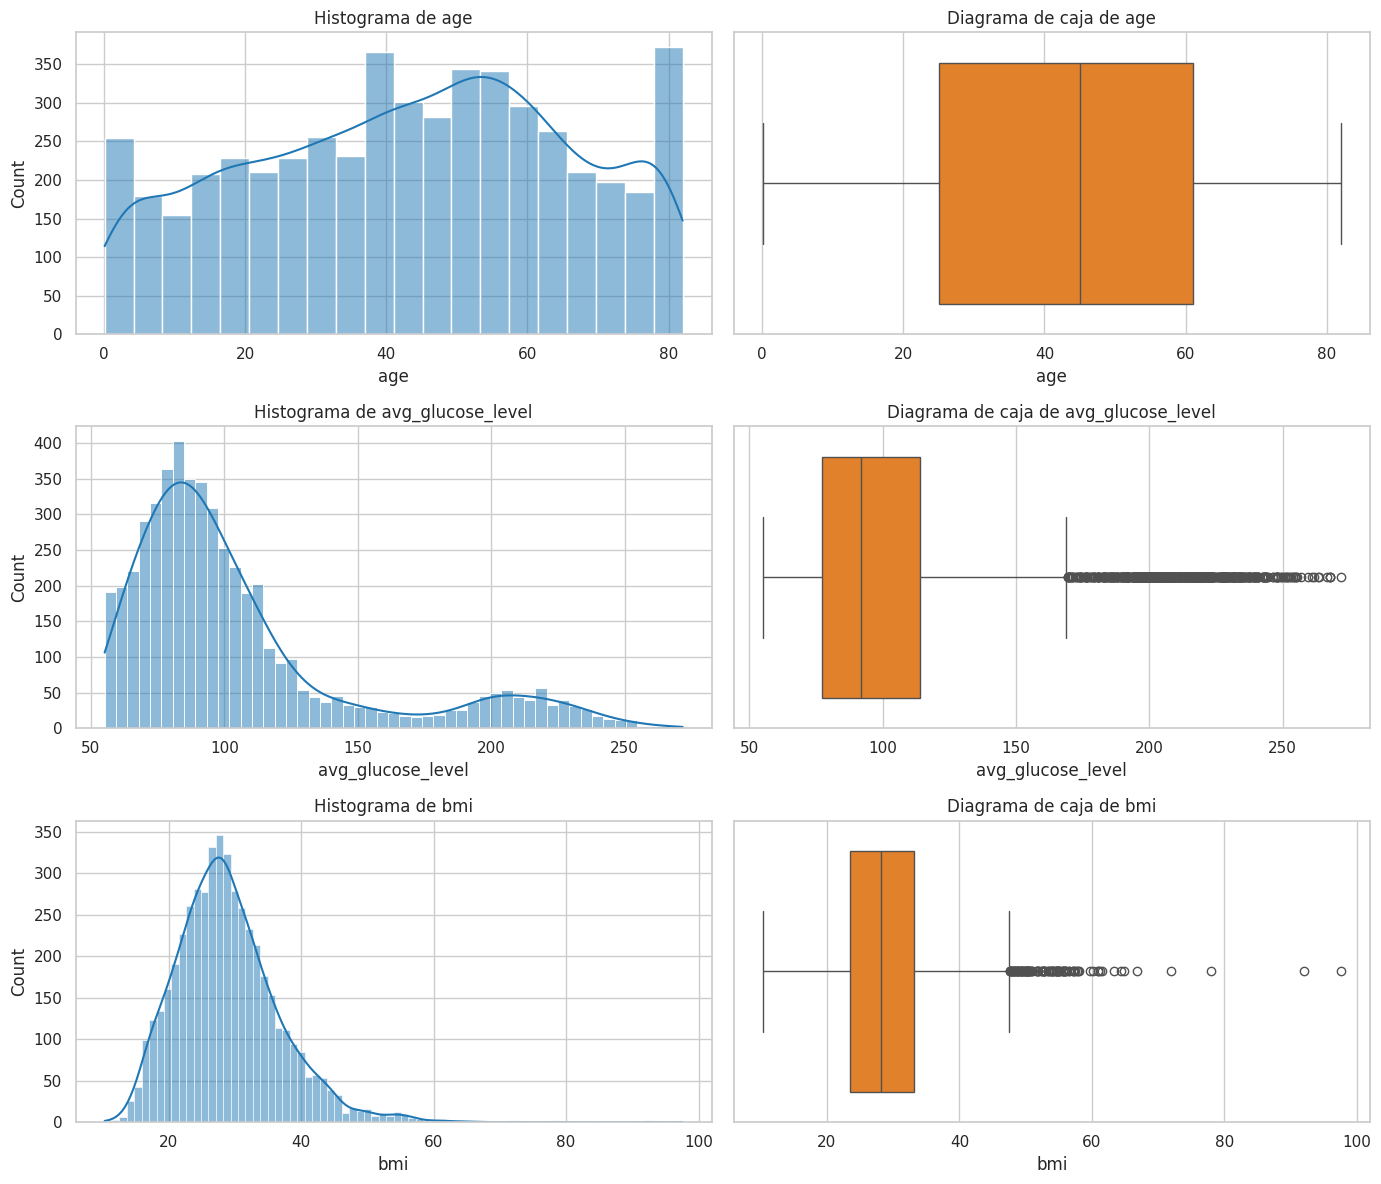
\includegraphics[width=\columnwidth]{../figures/eda_continuous.png}
\caption{Distribuciones e identificacion de valores atipicos en variables continuas.}
\label{fig:eda_continuous}
\end{figure}

\begin{figure}[htbp]
\centering
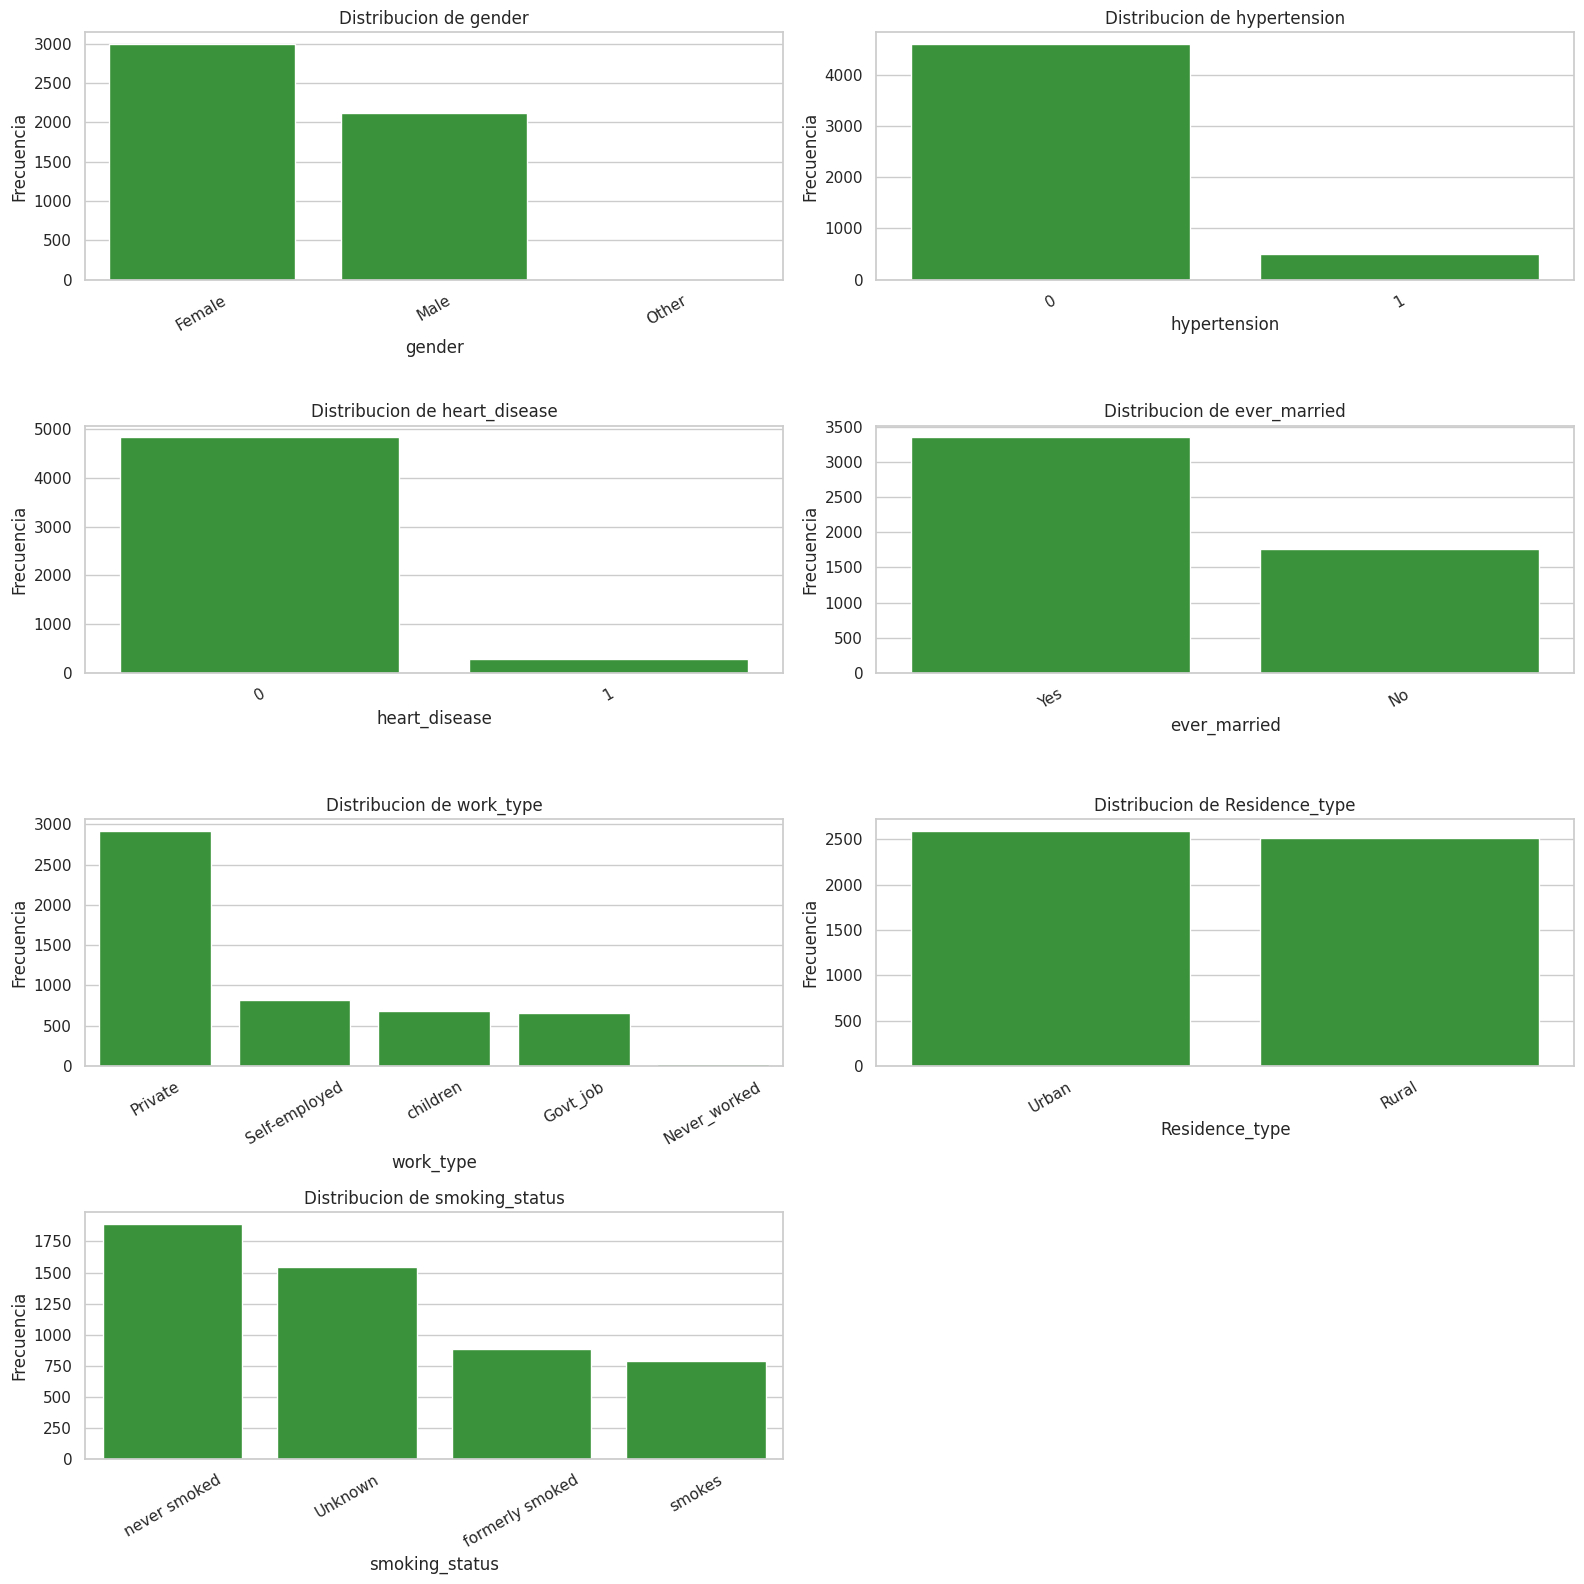
\includegraphics[width=\columnwidth]{../figures/eda_categorical.png}
\caption{Distribuciones de variables categoricas y balance de la variable objetivo.}
\label{fig:eda_categorical}
\end{figure}

\subsection{Preprocesamiento}
El flujo de preprocesamiento combina imputacion por mediana para variables continuas, imputacion por moda para variables categoricas, codificacion \texttt{OneHotEncoder} y normalizacion con \texttt{StandardScaler}. Esta secuencia se implemento mediante \texttt{Pipeline} y \texttt{ColumnTransformer}, garantizando consistencia entre entrenamiento y prueba.

\subsection{Modelos base}
Los modelos base fueron regresion logistica y Gaussian Naive Bayes. Ambos se entrenaron sobre la misma particion entrenamiento-prueba con muestreo estratificado, de modo que la proporcion de la clase objetivo se mantuviera estable en ambos subconjuntos.

\subsection{Diagnostico de la regresion logistica inicial}
Tras ejecutar el modelo logistico base, se analizaron sus metricas mas alla de la exactitud. El objetivo de esta etapa fue verificar si el clasificador era capaz de detectar la clase positiva o si simplemente aprendia a favorecer la clase mayoritaria.

\subsection{Regresion logistica ajustada}
El ajuste metodologico incorporo \texttt{class\_weight="balanced"} y una seleccion de umbral sobre un conjunto de validacion derivado del conjunto de entrenamiento. Esta decision permitio mantener intacto el conjunto de prueba para la comparacion final y evitar fuga de informacion.

\subsection{Metricas de evaluacion}
Las metricas consideradas fueron exactitud, \textit{balanced accuracy}, precision, recall, especificidad y F1-score. Adicionalmente, se analizaron las matrices de confusion para cuantificar verdaderos positivos, verdaderos negativos, falsos positivos y falsos negativos.

\subsection{Implementacion computacional}
La implementacion se realizo en Python con \texttt{pandas}, \texttt{numpy}, \texttt{matplotlib}, \texttt{seaborn} y \texttt{scikit-learn} \cite{b2}. El flujo completo se desarrollo en un notebook reproducible desde el cual se generaron las figuras utilizadas en este articulo.

\section{Resultados y discusion}
\subsection{Resultados del experimento base}
La Tabla~\ref{tab:baseline_results} resume el comportamiento de los dos modelos base. La regresion logistica obtuvo una exactitud muy alta, 0.952, pero ese resultado estuvo acompanado por un recall de apenas 0.020 y un F1-score de 0.039. Por el contrario, GaussianNB alcanzo un recall de 0.980, aunque con muy baja precision y una exactitud de solo 0.323.

\begin{table}[htbp]
\caption{Resultados del experimento base}
\label{tab:baseline_results}
\centering
\begin{tabular}{|l|c|c|c|c|}
\hline
\textbf{Modelo} & \textbf{Accuracy} & \textbf{Precision} & \textbf{Recall} & \textbf{F1-score} \\
\hline
Regresion logistica base & 0.952 & 1.000 & 0.020 & 0.039 \\
GaussianNB & 0.323 & 0.066 & 0.980 & 0.124 \\
\hline
\end{tabular}
\end{table}

La Fig.~\ref{fig:cm_baseline} confirma esta lectura. La regresion logistica base clasifico correctamente 972 casos negativos, pero solo detecto 1 de los 50 casos positivos, lo que muestra un sesgo extremo hacia la clase mayoritaria. En contraste, GaussianNB identifico 49 de 50 casos positivos, pero genero 691 falsos positivos, lo que limita fuertemente su utilidad practica.

\begin{figure}[htbp]
\centering
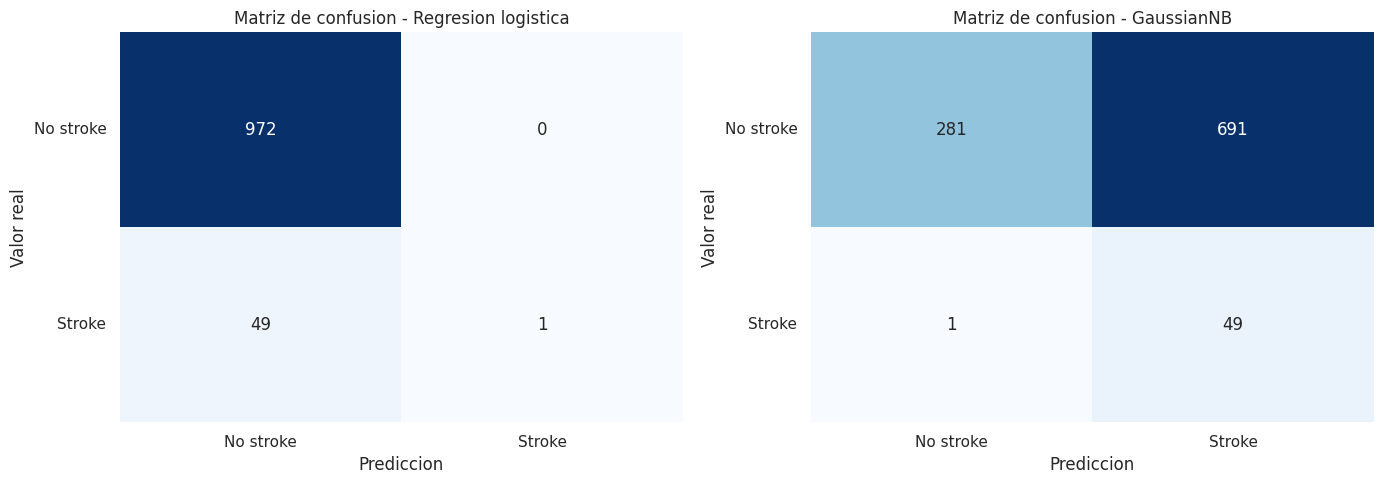
\includegraphics[width=\columnwidth]{../figures/cm_baseline_models.png}
\caption{Matrices de confusion de los modelos base.}
\label{fig:cm_baseline}
\end{figure}

\subsection{Justificacion del cambio metodologico}
Los resultados del experimento base muestran que la exactitud no es suficiente para seleccionar el mejor clasificador en este problema. Aun cuando la regresion logistica base parece superior por \textit{accuracy}, en realidad deja pasar casi todos los casos positivos, lo que resulta inaceptable en un contexto clinico. Esta evidencia justifica la modificacion del procedimiento original mediante ponderacion de clases y ajuste del umbral de decision.

\subsection{Resultados del modelo ajustado}
La regresion logistica balanceada con umbral 0.50 incremento el numero de verdaderos positivos de 1 a 40 y redujo los falsos negativos de 49 a 10. Este ajuste elevo el recall a 0.800, aunque introdujo 249 falsos positivos. Posteriormente, la version con umbral optimizado mantuvo el mismo recall de 0.800, pero redujo los falsos positivos a 216 y aumento los verdaderos negativos a 756, mejorando asi la especificidad, la precision y el F1-score.

\subsection{Comparacion final entre modelos}
La Tabla~\ref{tab:final_results} presenta la comparacion cuantitativa final. La regresion logistica balanceada con umbral optimizado obtuvo la mejor combinacion global entre recall, especificidad y F1-score. Aunque GaussianNB mantuvo el recall mas alto, 0.980, su precision de 0.066 y su especificidad de 0.289 reflejan un volumen excesivo de falsas alarmas.

\begin{table}[htbp]
\caption{Comparacion final entre modelos}
\label{tab:final_results}
\centering
\resizebox{\columnwidth}{!}{%
\begin{tabular}{|l|c|c|c|c|c|c|}
\hline
\textbf{Modelo} & \textbf{Accuracy} & \textbf{Bal. Acc.} & \textbf{Precision} & \textbf{Recall} & \textbf{Specificity} & \textbf{F1-score} \\
\hline
Logistica base & 0.952 & 0.510 & 1.000 & 0.020 & 1.000 & 0.039 \\
Logistica balanceada 0.50 & 0.747 & 0.772 & 0.138 & 0.800 & 0.744 & 0.236 \\
Logistica balanceada optima & 0.779 & 0.789 & 0.156 & 0.800 & 0.778 & 0.261 \\
GaussianNB & 0.323 & 0.635 & 0.066 & 0.980 & 0.289 & 0.124 \\
\hline
\end{tabular}}
\end{table}

La Fig.~\ref{fig:cm_final} sintetiza visualmente esta comparacion. La regresion logistica balanceada con umbral optimizado preserva 40 verdaderos positivos y 10 falsos negativos, igual que la variante balanceada con umbral 0.50, pero reduce falsos positivos de 249 a 216. Esta mejora confirma que el cambio metodologico no fue arbitrario, sino una respuesta directa a la falla observada en el modelo logistico inicial.

\begin{figure}[htbp]
\centering
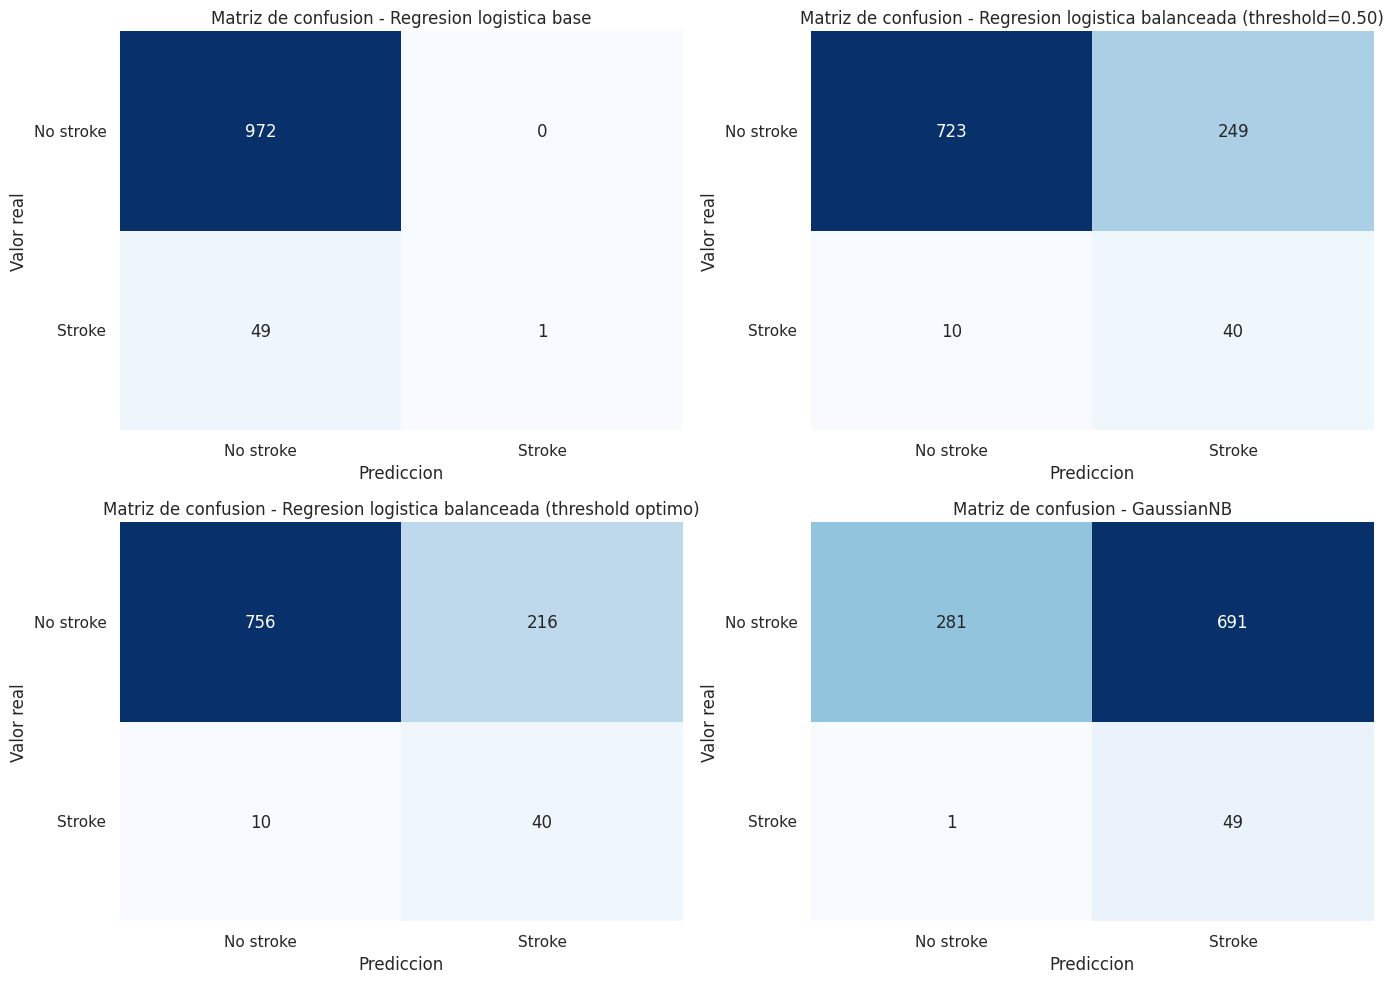
\includegraphics[width=\columnwidth]{../figures/cm_final_models.png}
\caption{Matrices de confusion de la comparacion final entre modelos.}
\label{fig:cm_final}
\end{figure}

\subsection{Limitaciones del estudio}
El estudio presenta al menos tres limitaciones. En primer lugar, el conjunto de datos esta severamente desbalanceado, lo que obliga a interpretar los resultados con especial atencion a la clase positiva. En segundo lugar, la comparacion se realizo sobre un unico dataset, por lo que la validez externa del experimento es limitada. En tercer lugar, aunque la regresion logistica balanceada mejoro claramente el desempeno, todavia mantiene una precision modesta, lo que sugiere espacio para incorporar remuestreo, calibracion de probabilidades o modelos adicionales en trabajos futuros.

\section{Conclusiones}
Este trabajo mostro que la regresion logistica base no era adecuada para la deteccion de stroke, a pesar de su alta exactitud, debido a que practicamente ignoraba la clase minoritaria. La comparacion con GaussianNB evidencio el problema opuesto: un recall muy alto, pero con un volumen excesivo de falsos positivos.

La incorporacion de ponderacion de clases y ajuste de umbral permitio transformar la regresion logistica en un modelo mas util para el problema. En particular, la regresion logistica balanceada con umbral optimizado alcanzo una exactitud de 0.779, una \textit{balanced accuracy} de 0.789, un recall de 0.800 y un F1-score de 0.261, constituyendo el mejor compromiso entre sensibilidad y control de falsas alarmas.

En consecuencia, la mejor alternativa de esta iteracion no fue el modelo con mayor exactitud ni el modelo con mayor recall aislado, sino aquel que mostro el balance mas razonable entre recall, especificidad y F1-score. Como trabajo futuro, resulta pertinente evaluar estrategias de remuestreo, calibracion y modelos adicionales para seguir mejorando la deteccion de stroke.

\begin{thebibliography}{00}
\bibitem{b1}
F. Soriano, ``Stroke Prediction Dataset,'' Kaggle, 2021. [Online]. Available: \url{https://www.kaggle.com/datasets/fedesoriano/stroke-prediction-dataset}

\bibitem{b2}
F. Pedregosa \textit{et al.}, ``Scikit-learn: Machine Learning in Python,'' \textit{Journal of Machine Learning Research}, vol. 12, pp. 2825--2830, 2011.

\bibitem{b3}
T. Hastie, R. Tibshirani, and J. Friedman, \textit{The Elements of Statistical Learning}, 2nd ed. New York, NY, USA: Springer, 2009.

\bibitem{b4}
World Health Organization, ``The top 10 causes of death,'' 2024. [Online]. Available: \url{https://www.who.int/news-room/fact-sheets/detail/the-top-10-causes-of-death}
\end{thebibliography}

\end{document}
